\section{Discussion}
\label{sec:dis}
\subsection{The onset stage of frequency chirping}
Recalling cell definition, it is a local reference frame that tracks the local resonant particle at rest.
However, when the chirping begins, it is hard to follow the resonance particle precisely since the local resonance changes all the time.
To reduce the complexity of the dynamics system without losing any generality, we here consider the initial time stage of the chirping problem, i.e., the onset problem.
The variation of wave frequency is considerably small in the onset stage of the instability. 
Thus, the resonance frame is approximately centered at the most unstable frequency $\omega_l$ and the corresponding wave number $k_l$ obtained from the linear wave dispersion.
By simply replacing $k_i$, $\omega_i$ by $\omega_l$ and $k_l$ in the related parameters and equations, we can greatly reduce the motion equation.
For the perturbed motion, the parameter $alpha$ is greatly reduced. Since the most unstable frequency is a temporospatial constant, $\partial \omega/\partial t$ is vanished in Eq.~(\ref{eq.alp1}).
While the exact time derivative of $k_l$ still has dependence on $s$, i.e.,
\begin{equation}
    \frac{\mathrm{d}k_l}{\mathrm{d}t}  = v_r \frac{\partial k_l}{\partial s}~.
\end{equation}
According to the linear dispersion
\begin{equation}
    c^2 k_l^2=\omega_l^2+\frac{\omega_{pe}^2\omega_l }{\omega_{ce}-\omega_l}~,
\end{equation}
do differentiate on both sides with respect to $s$ yields
\begin{equation}
    \begin{aligned}
    2 c^2 k_l \frac{\partial k_l}{\partial s}&=\left(2 \omega_l+\frac{\omega_{ce} \omega_{pe}^2}{\left(\omega_{ce}-\omega_l\right)^2}\right) \frac{\partial \omega_l}{\partial s}-\frac{\omega_l \omega_{pe}^2}{\left(\omega_{ce}-\omega_l\right)^2} \frac{\partial \omega_{ce}}{\partial s}
    \\
    & = -\frac{\omega_l \omega_{pe}^2}{\left(\omega_{ce}-\omega_l\right)^2} \frac{\partial \omega_{ce}}{\partial s}~,
    \end{aligned}
\end{equation}
i.e.,
\begin{equation}
    \frac{\partial k_l}{\partial s} = -\frac{\omega_l \omega_{pe}^2}{2 c^2 k_l \left(\omega_{ce}-\omega_l\right)^2} \frac{\partial \omega_{ce}}{\partial s}~.
\end{equation}
Note that we neglect the dependence of $\omega_{pe}$ on $s$.
\begin{equation}
    \begin{aligned}
        \frac{\partial k_l}{\partial s} &=- \frac{c^2 k_l^2 - \omega_l^2}{2 c^2 k_l^2}\frac{k_l}{(\omega_{ce}-\omega_l)} \frac{\partial \omega_{ce}}{\partial s}
        \\
        &=-\frac{1}{v_r} (\frac{1}{2} - \frac{\omega_l^2}{2c^2 k_l^2}) \frac{\partial \omega_{ce}}{\partial s}
        \\
        &\simeq \frac{1}{2v_r}\frac{\partial \omega_{ce}}{\partial s}~.
    \end{aligned}
\end{equation}
The phase velocity is close to the speed of light for the whistler dispersion at the frequency of interest, thus we have the above approximation.

The onset condition finally gives 
\begin{equation}\label{eq.alp1}
   \alpha \simeq \frac{k_l}{\omega_b^2}\left(\mathcal{J}-\frac{\Pi_i}{2}\right) \frac{\mathrm{d} \omega_{c e}}{\mathrm{~d} s}
    \end{equation}

In addition, with the onset condition, the motion equation (\ref{eq.m3}) for $\mathcal{J}$ reduces to
\begin{equation}
        \frac{\mathrm{d}\mathcal{J}}{\mathrm{d}t} \simeq  \frac{m_e(\omega_l - \omega_{ce})}{k_l^3} \frac{\mathrm{d} k_l}{\mathrm{d} t} + \frac{m_e(\omega_l - \omega_{ce})}{k_l^3} \frac{\partial \omega_{ce}}{\partial s_i}  +\frac{\mathcal{J}}{k_l}\frac{\partial \omega_{ce}}{\partial s_i}~.
\end{equation}
Multiplying $\omega_l - \omega_{ce}$ on both sides to construct $v_r$ on the spatial derivative of $\omega_{ce}$ that change the spatial derivative to exact time derivative, i.e., 
\begin{equation}
    (\omega_l - \omega_{ce}) \frac{\mathrm{d}\mathcal{J}}{\mathrm{d}t} \simeq  \frac{m_e(\omega_l - \omega_{ce})^2}{k_l^3} \frac{\mathrm{d} k_l}{\mathrm{d} s_i} + \frac{m_e(\omega_l - \omega_{ce})}{k_l^2} \frac{\mathrm{d} \omega_{ce}}{\mathrm{d} t} + \mathcal{J}\frac{\mathrm{d} \omega_{ce}}{\mathrm{d} t}~.
\end{equation}
Further using the identity $\mathrm{d}\omega_l/\mathrm{d}t \equiv 0$, we obtain the following relation
\begin{equation}
    (\omega_l - \omega_{ce}) \frac{\mathrm{d}\mathcal{J}}{\mathrm{d}t} + \mathcal{J}\frac{\mathrm{d}}{\mathrm{d} t}(\omega_l - \omega_{ce}) \simeq - m_e\left((\omega_l - \omega_{ce})^2 \frac{\mathrm{d}}{\mathrm{d} t}\frac{1}{2 k_l^2} + \frac{1}{2 k_l^2} \frac{\mathrm{d}}{\mathrm{d} t}(\omega_l - \omega_{ce})^2\right)~.
\end{equation}
The equation is clearly to be analytically integrated, and yields
\begin{equation}\label{eq.Jcons}
    (\omega_l - \omega_{ce})\mathcal{J} +  \frac{m_e(\omega_l - \omega_{ce})^2}{2k_l^2} = \mathrm{Const.}
\end{equation}
The constant for each cell is determined by the initial choice of $\mathcal{J}$, which give the entire information of the dynamics on the slowly varying scale along the magnetic field line.

\subsection{The adiabatic theory}
%solve current integral and obtain the chirping law
In the previous section, we obtain the nonlinear current from the velocity moment of the perturbed distribution function. 
The current dominates the nonlinear behavior of the chorus chirping process, and under certain condition, we can simplify the phase space integral and show qualitatively how does the current evolves.
At the nonlinear stage, the distribution function of the trapped electrons forms a hole in the phase space, and we consider its deviation from the unperturbed distribution $\Delta f$, i.e., the depth of the hole.
Since the equilibrium distribution does not contribute to the current, the nonlinear current is directly determined by $\Delta f$, 

%the adiabatic invariant 
For those electrons trapped by the slowly varying wave envelope and circling around in the phase space, we can define the adiabatic invariant at a given $s_i,\mathcal{J}$,
\begin{equation}\label{eq.def_I}
    \mathcal{I} = \frac{1}{2\pi} \oint \Omega(H_i,\xi,t) \mathrm{d} \xi~,
\end{equation}
where the momentum $\Omega$ is the function of local Hamiltonian.
%and the distribution expansion
The depth of the hole can be written as the function of the adiabatic invariant, i.e., $\Delta f(s_i,\mathcal{J},\mathcal{I},\xi,t)$.

Now we replace $f$ by $\Delta f$ in the current integral in Eq. (\ref{eq.nonlinear_J}) and directly change the integral to 
\begin{equation}
    j_p(s_i,t) \approx - \int\mathrm{d} \mathcal{J} \sqrt{2 m_e \omega_{ce} (\mathcal{J} + \Pi_i(t))} \int_0^{\mathcal{I}_{\mathrm{s p x}}}  \mathrm{d}\mathcal{I}  \oint \mathrm{d}\psi  \Delta f(s_i,\mathcal{J},\mathcal{I},\xi,t)e^{\imath \xi}  ~,
\end{equation}
Note that $\Omega$ in the square root can be neglect since $\Omega \simeq 0$.
The differential element $\mathrm{d}\xi\mathrm{d}\Omega$ is changed to $\mathrm{d}\mathcal{I}\mathrm{d}\psi$, where $\psi$ is the angle variable of $\mathcal{I}$.
From the Jacobi of the differential element, the integral over $\psi$ 
\begin{equation}
      \oint f \mathrm{d}\psi = \oint f \frac{\mathrm{d}\Omega}{\mathrm{d}\mathcal{I}}\mathrm{d}\xi = \frac{\partial H}{\partial \mathcal{I}} \oint f \frac{\mathrm{d}\Omega}{\mathrm{d} H}\mathrm{d}\xi = \dot{\psi}\oint \frac{f}{\Omega} \mathrm{d}\xi = 2 \pi \langle f \rangle
\end{equation}
where $\langle\cdots\rangle$ denotes the bounce average following the definition in ref. \cite{berk1999}.
Thus the current integral becomes
\begin{equation}\label{eq.adiabatic_current}
    j_p(s_i,t) \approx -  {2\pi} \int\mathrm{d} \mathcal{J}  \sqrt{2m_e\omega_{ce} (\mathcal{J} + \Pi_i(t))} \int_0^{\mathcal{I}_{\mathrm{s p x}}}\mathrm{d}\mathcal{I}  \langle \Delta f(s_i,\mathcal{J},\mathcal{I},\xi,t)e^{\imath \xi} \rangle  ~.
\end{equation}

For the adiabatic regime, the characteristic scales should vary considerably slowly compared to the wave trapping scale.
There exists a small scale $\epsilon$ satisfies \cite{berk1999}
\begin{equation}
    \epsilon \equiv \mathrm{max}\left(\ddot{\omega}/\omega_b^3, \dot{\omega}/\omega_b^2, \omega_b/\omega \right) \ll 1~,
\end{equation}
Here, $\omega$ is the frequency deviation from the resonance center in our context.
For the chorus wave field, the frequency, and other quantities change slowly in one bounce period, satisfying the first and the second inequalities. The last term requires the frequency chirped a notable distance, i.e., the nonlinear stage, where the hole has been separated from the equilibrium.
$\Delta f$ can be expanded in powers of $\epsilon$ and follows the derivation in ref. \cite{berk1999}, the bounce averages in Eq.~(\ref{eq.adiabatic_current}) are
\begin{equation}
    \begin{aligned}
    \langle\Delta f \sin \xi \rangle &\simeq \alpha \Delta f_0 ~, \\ 
    \langle \Delta f \cos \xi \rangle &\simeq  \Delta f_0 \langle \cos \xi \rangle ~.
    \end{aligned}
\end{equation}
%approximation 2, I is constant over trapped region
Moreover, we further assume that $\Delta f_0$ is independent with $\mathcal{I}$, which indicates the depth of the hole is flat within the enclosed phase space region, i.e., the water bag approximation \cite{omura_theory_2008,hezaveh2021}. Therefore, the integral over $\mathcal{I}$ only depend on the $\mathcal{I}_\mathrm{spx}$ which is the one on the separatrix. 
According to equation (\ref{eq.def_I}), the integral becomes
\begin{equation}
    \int^{\mathcal{I}_\mathrm{s p x}}_0 \mathrm{d}\mathcal{I} = \mathcal{I}_\mathrm{s p x} \equiv \oint_\mathrm{s p x} \Omega (\xi) \mathrm{d} \xi~,
\end{equation}
where the boundary trapped particle phase space hole can be analytically given,
\begin{equation}
    \Omega(\xi) = \pm \frac{\omega_b}{k^2} \sqrt{2 (e_\mathrm{spx}-\cos \xi - \alpha \xi)}~,
\end{equation}
and $e_{spx}$ denotes the Hamiltonian on the separatrix. Now we define two functions of $\alpha$
\begin{equation}\label{eq.function}
    \begin{aligned}
        m_{spx}(\alpha) & \equiv \langle \cos \xi \rangle  \mathcal{I}_\mathrm{spx} = \frac{\sqrt{2} \omega_b}{k^2} \oint_\mathrm{s p x} \mathrm{d} \xi \cos \xi \sqrt{e_\mathrm{s p x}-\cos \xi-\alpha \xi} 
        \\
        n_{spx}(\alpha) & \equiv \alpha \mathcal{I}_\mathrm{spx} = \alpha \frac{\sqrt{2} \omega_b}{k^2} \oint_\mathrm{s p x} \mathrm{d} \xi \sqrt{e_\mathrm{s p x}-\cos \xi-\alpha \xi}~,
    \end{aligned}
\end{equation}
and yield current 
\begin{equation}\label{eq.adi_J}
    j_p(s_i,t) \approx \frac{4 \pi \omega_b}{k^2} \left(m_\mathrm{s p x}+\imath ~ n_\mathrm{s p x}\right) \int \mathrm{d} \mathcal{J} \sqrt{m_e \omega_{c e}(\mathcal{J}+\Pi_i(t))} \Delta f(\mathcal{J},s_i,t) ~.
\end{equation}
%the nonlinaer currnet and the chirping rate ...
%differnece with omura 
%process approxiamtion strict follows adiabatic approximation
%why the hole is oblique
%alpha value should small to validate approximation
%figure

\begin{figure}
    \centering
    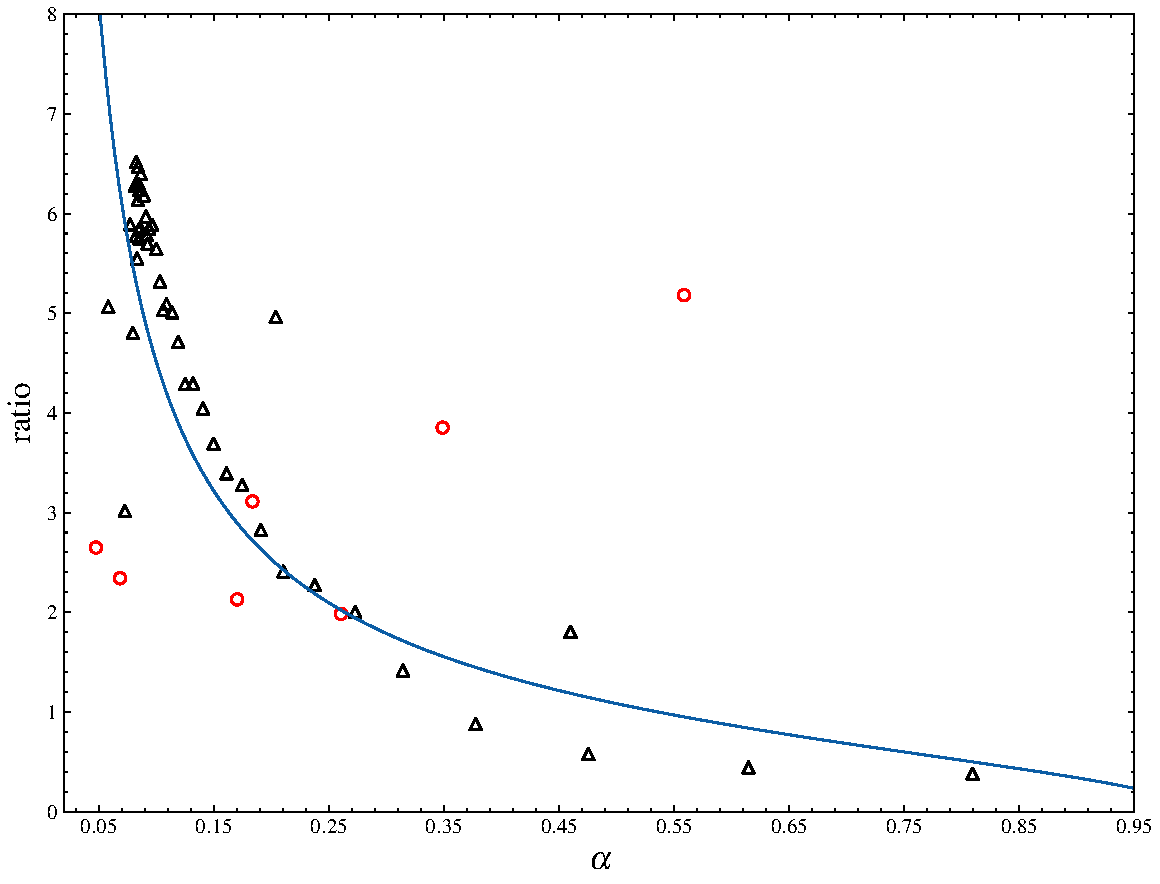
\includegraphics[scale=0.5]{img/fig_adiabatic.pdf}
    \caption{The current ratio with respect to the inhomogeneous parameter $\alpha$. The scattered points are from numerical simulation in ref. \cite{zheng2023b}, while the solid curves denotes the results from adiabatic approximation.}
    \label{fig.adiabatic}
\end{figure}


The temporospatial evolution of the nonlinear current only depends on the integral over the slowly varying scale $\mathcal{J}$, and an inhomogeneity parameter $\alpha$, defined in Eq. (\ref{eq.alp0.5}). 
The $\mathcal{J}$ integral can be solved further harnessing the adiabatic motion of the trapped particle along the magnetic field line, similar to the previous work \cite{summers2012}. 
However, we first need to show the validity of the adiabatic approximation. 


To do so, we examine the ratio of the imaginary and real component of $j_p$, i.e., $\mathrm{real}(j_p)/\mathrm{imag}(j_p)$. The dependence on the integral is removed and the ratio only depends on the value $\alpha$.
From the adiabatic theory, Eqs. (\ref{eq.adi_J}) and (\ref{eq.function}), we obtain the current ratio as function of $\alpha$ and show the relation in Fig. \ref{fig.adiabatic}.
Also, base on the above-mentioned Vlasov theory, we performed a corresponding numerical simulation \cite{zheng2023b}, in which the current is obtained directly from Eq. (\ref{eq.nonlinear_J}).
The corresponding $\alpha$ is obtained from the definition in Eq. (\ref{eq.alp0.5}) using the simulation data.
The comparison of the current ratio obtained with the adiabatic results show two different behavior.
The in the wide spatial range far from the magnetic equator (triangle shape), the simulation results well agree with the adiabatic approximation. While in the equator region (circle shape), the adiabatic approximation ceases to be valid. 
This indicates a rapid variation of the phase space in the equator region, which is related to the generation of the nonlinear chorus wave.